\documentclass[12pt,fleqn]{article}
\usepackage{
  amsmath,
  amssymb,
  booktabs,
  geometry,
  graphicx,
  microtype,
  parskip,
  caption,
}
\usepackage[shortlabels]{enumitem}

\geometry{margin=3cm}

% equation line spacing
\setlength{\jot}{0.5cm}

% meta data
\newcommand{\chapter}{10.1, 10.2, 11.3}
\newcommand{\authorname}{Amo DelBello}
\newcommand{\classdescription}{MATH 1350-D2}
\newcommand{\classname}{Introduction to Statistics, Fall 2022}
\newcommand{\assignment}{\chapter\ Book Assignment}

% \newcommand{\problemtenone}[1]{\vspace{5ex}\section*{\chapter-#1}}
\newcommand{\problemtenone}[1]{\vspace{5ex}\section*{10.1-#1}}
\newcommand{\problemtentwo}[1]{\vspace{5ex}\section*{10.2-#1}}
\newcommand{\problemeleventhree}[1]{\vspace{5ex}\section*{11.3-#1}}
\newcommand{\thead}[1]{\textnormal{\textbf{#1}}}
\newcommand{\tvspace}{\vspace{.25cm}}

\title{\classdescription\ \\ \classname\ \\ $\ $ \\ \assignment}
\author{\authorname}
\date{\today}


\begin{document}

\maketitle


\problemtenone{4}
\begin{enumerate}[label=\alph*)]
\item -1
\item 0.746
\item 0.268
\item 0.992
\item 1
\end{enumerate}


\problemtenone{7}
The value for $r = 0.1174$ is pretty far from 1 or -1. Therefore there does not sufficient evidence to support the claim that there is a linear correlation between the weights.

\pagebreak
\problemtenone{9}
\begin{enumerate}[label=\alph*.]
\item
  \begin{figure}[ht]
    \centering
    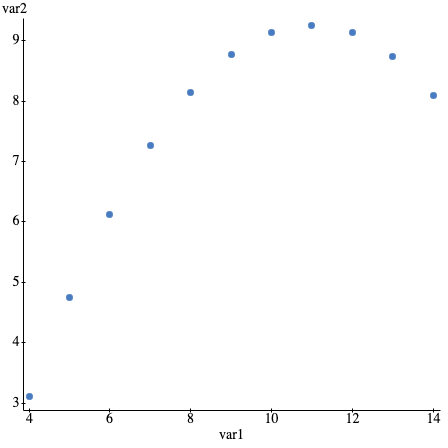
\includegraphics[width=9cm]{assets/scatterplot-1.png}
  \end{figure}

\item $r = 0.816$, The problem doesn't specify a value for $\alpha$ so I will just use 0.05. As the P-Value $0.002 \le \alpha$, the claim of linear correlation is supported.

\item If part (b) was completed without of scatterplot the fact that the data has a non-linear pattern would not be known.
\end{enumerate}


\problemtenone{10}
\pagebreak
\begin{enumerate}[label=\alph*.]
\item
  \begin{figure}[ht]
    \centering
    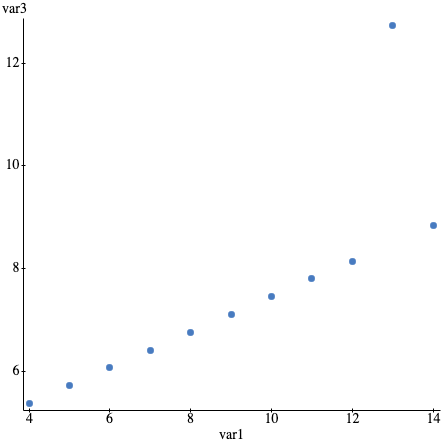
\includegraphics[width=9cm]{assets/scatterplot-2.png}
  \end{figure}

\item $r = 0.816$, The problem doesn't specify a value for $\alpha$ so I will just use 0.05. As the P-Value $0.002 \le \alpha$, the claim of linear correlation is supported.

\item If part (b) was completed without of scatterplot the fact that the data has an outlier affecting it's $r$ value would not be known.
\end{enumerate}


\problemtenone{17}
$r = 0.591$, P-Value = 0.294

Using an $\alpha = 0.05$, and as P-Value > $\alpha$, we conclude that there is not sufficient evidence to support the claim that there is a linear correlation between shoe print lengths and heights. It does not appear that police can use foot length to estimate the height of a male.


\pagebreak
\problemtentwo{10}
\begin{figure}[ht]
  \centering
  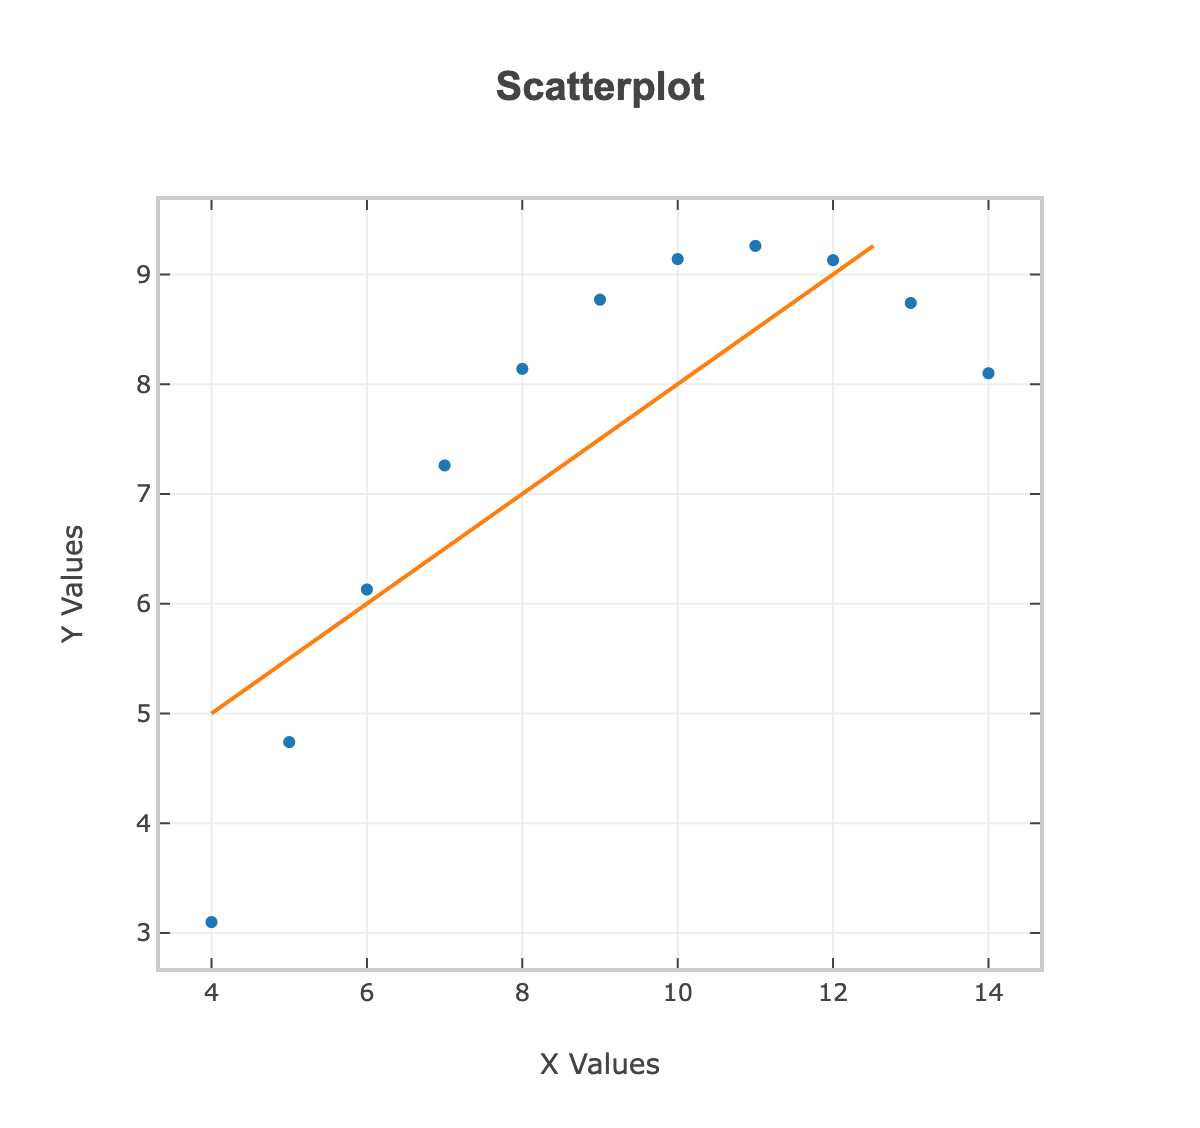
\includegraphics[width=12cm]{assets/scatterplot-3.png}
\end{figure}

\begin{align*}
  \hat{y} &= b_0 + b_1x \\
  \hat{y} &= 3.001 + 0.5x
\end{align*}
A characteristic of the data that is ignored by the regression line is the fact that the data has a non-linear pattern.


\problemtentwo{15}
Regression equation: $\hat{y} = -0.0111 + 1.01x$
\begin{align*}
  \hat{y} &= -0.0111 + 1.01 * 3.00 \\
  \hat{y} &= \$3.02
\end{align*}
The best predicted fare of \$3.02 is not likely to be implemented because rarely do we see prices that do not end at the typical numbers of ``00'', ``95'', or ``99.''


\problemtentwo{17}
Regression equation: $\hat{y} = 125.407 + 1.73x$

The regression equation is not a good model so the best predicted value of y is the value of $\bar{y}$ which is 177.3 cm.

As we are using the mean of y instead of the regression equation, the result would not be helpful to police crime scene investigators in trying to describe the male.


\problemeleventhree{11}
Using Statdisk One-Way Analysis of Variance, I determined that the P-Value for the three miles is 0.00003. As the P-Value $< \alpha$ of 0.05 we reject the null hypothesis that $H_0: \mu_1 = \mu_2 = \mu_3$. It appears that the third mile took longer than the other two so it would be reasonable to assume that mile had a hill.


\problemeleventhree{12}
Using Statdisk One-Way Analysis of Variance, I determined that the P-Value for the arsenic levels in rice for the three states is 0.00000. As the P-Value $< \alpha$ of 0.05 we reject the null hypothesis that $H_0: \mu_1 = \mu_2 = \mu_3$.

Instead of concluding that the arsenic levels in Texas are higher, it may make more sense to conclude that the arsenic levels in California are lower. There seems to be more of a difference between the California rice from the Arkansas and Texas rice, rather than a difference between Texas and the other too. It may be more correct to say that California's rice poses the least health problem.


\problemeleventhree{15}
Using Statdisk One-Way Analysis of Variance, I determined that the P-Value for the counts of chocolate chips from the three different types of cookies to be 0.00000. As the P-Value $< \alpha$ of 0.05 we reject the null hypothesis that $H_0: \mu_1 = \mu_2 = \mu_3$. However, it does not appear that the mean of chocolate chips in the reduced fat cookies is lower. In fact they are actually higher than the ``chewy'' variety:

  \begin{tabular}{@{}lll@{}}
    \thead{Regular} & \thead{Chewy} & \thead{Reduced Fat} \\
    \toprule
    23.95 & 19.09 & 19.6 \\
    \bottomrule
  \end{tabular}
  \vspace{.25cm}



\end{document}
%%% Local Variables:
%%% mode: latex
%%% TeX-master: t
%%% End:
